\section{Computational experiments and results}
\label{chap:census}

\subsection{A census of prime spaces induced by small g-blinks}
\label{sec:census}

\newcommand{\kpu}{\,$k$-prime-unavoidable }
\newcommand{\npu}[1]{\,$#1$-prime-unavoidable }
\newcommand{\Rk}{{\cal R}_k }
\newcommand{\Rkl}{{\cal R}'_k}

In Section~\ref{sec:towardsACensusOfPrimeSpacesInducedBySmallBlinks}
we saw that if we have a set with all representative g-blinks with
$\,\,\leq k \,\,$ g-edges, then all spaces induced by blinks with
$\,\,\leq k \,\,$ edges are there. Even though, for any fixed $k \geq
1$ this set is finite, we would like to search for spaces in an
even smaller set and not lose any space. This may be done if we
believe in the following reasonable conjecture.

\begin{conjecture} \label{conj:noCompositeHasFewerEdgesThanItsMinimalPrimeSum}
Let a space $S$ be the connected sum of prime spaces $A$ and $B$.
If the minimal blink presentations for $A$ and $B$ have respectively $n_A$ and
$n_B$ edges, then $n_S$, the number of edges for the minimal blink presentation
of $S$, satisfies  $n_S = n_A + n_B$.
\end{conjecture}

A {\em minimal blink for a space} is a blink that
has the same number of edges or fewer edges than any other blink
presentation for that space. A {\em prime space} is one that cannot
be expressed by a connected sum of two or more spaces
different from $\mathbb{S}^3$. A {\em composite space} is a space
that is not prime, i.e. one space that can be expressed by a connected sum of
two or more spaces different from $\mathbb{S}^3$. A blink presentation for any composite space
is obtained by drawing the blinks of each of its prime pieces
separately in the same drawing: a red-green plane graph with more than one
connected component. This construction clearly defines an upper bound for
the minimal number of edges of the composite space: the sum of
the number of edges of a minimal blink for each of its
prime pieces. Suppose space $S$ is the connected sum of $n$ prime
spaces, a minimal blink for $S$ with $n$ connected
components satisfies this upper bound, otherwise there would be
a blink for one of its prime pieces with fewer edges than its minimum
number of edges which is a contradiction. The only
possibility that remains to the conjecture to be false is
a blink presentation with less than $n$ components. On the other
hand we have,

\begin{proposition} \label{prop:primeIsSufficient}
If Conjecture~\ref{conj:noCompositeHasFewerEdgesThanItsMinimalPrimeSum} is true
then, knowing one minimal blink for each prime space that has a blink presentation
with $\leq k$ edges, it is possible to exhibit a minimal blink
for all spaces (composite or prime) that have a blink presentation with
$\leq k$ edges.
\end{proposition}
\begin{proof}
If $S$ is a prime space that has a blink with fewer than $k$ edges then,
by hypothesis, we already know one minimal blink for it. If $S$ is composite,
then exhibit together in a single drawing the minimal blink of all its prime
pieces. By the Conjecture~\ref{conj:noCompositeHasFewerEdgesThanItsMinimalPrimeSum}
this is a minimal blink for $S$.
\end{proof}

A consequence of Proposition~\ref{prop:primeIsSufficient} is that, if
Conjecture~\ref{conj:noCompositeHasFewerEdgesThanItsMinimalPrimeSum} is true, then
to identify all spaces that have a blink presentation with fewer than $k$ edges
it is sufficient to know only the prime spaces that have a blink
presentation with fewer than $k$ edges. So, in our experiment,
this is what we do. We focus only on prime spaces. We simplify our
computational effort by answering not what are all the spaces with
a blink presentation with fewer than $k$ edges, but what are all the
\underline{prime} spaces with a blink presentation with fewer than $k$
edges. So, we may reduce the set of representative g-blinks to
representative g-blinks that are prime or, in practice, that are
not easily shown composite.

Spaces have an orientation. If we swap the red-green edges of a
blink the effect on the induced space is its change of orientation.
So, any set of blinks $B$ that induces spaces $S$ may be easily
extended to a set of blinks $B'$ that induces $S$ and also the
changed orientation version of the spaces in $S$. The set $B'$ is
just $B$ plus the blinks of $B$ with the red-green edges swapped.
This leads us to the following definition: a {\em set of blinks} is
said to be {\em \kpu} if every space with a blink presentation with
$\,\,\leq k \,\,$ edges is induced by some blink in this set or a
red-green swapped version of some blink in this set. These notions
are analogously extended to g-blinks. A {\em set of g-blinks} is
said to be {\em \kpu} if every space with a g-blink presentation with
$\,\,\leq k \,\,$ g-edges is induced by some g-blink in this set or
a red-green g-edges swapped version of some g-blink in this set.

\newpage

What we mean concretely by the title of this section:
{\em a census of prime spaces induced by
g-blinks} is a triple \vspace{-0.3cm}$$(k,{\cal B},f:{\cal B}
\rightarrow \{1, \ldots, n\}),\vspace{-0.3cm}$$ where $k$ is a
positive integer, ${\cal B}$ is a \kpu set of g-blinks and $f$ is a
surjective function that maps each g-blink in ${\cal B}$ to an integer
in $\{1, \ldots, n\}$ satisfying the constraints: if $B_1,B_2 \in
{\cal B}$ induce the same space or induce the same space with
swapped orientations then $f(B_1) = f(B_2)$, else
$f(B_1) \neq f(B_2)$. Note that $f$ defines a partition of ${\cal B}$
into $n$ classes where the g-blinks in each class induce the same space
modulo orientation. For this reason we call $f$ the
{\em partition function} of the census. In view of this definition of a
census of prime spaces, the steps to build one are: (1) define $k$;
(2) define a \kpu set of g-blinks; (3) define the partition function $f$.

\subsection{A prime-unavoidable set of g-blinks: $U$}

To obtain a census of prime spaces induced by g-blinks with $\,\,\leq
k \,\,$ edges, a set of \kpu g-blinks is needed. Before defining the
specific way we did this generation it is good to say that in theory
what is needed to do is simple: enumerate all representative g-blinks up to size
$k$ and discard those that you can show that are composite or that are
not minimal. In practice we use some shortcuts to avoid a full
enumeration of all representative g-blinks.

The procedure we defined to obtain a \kpu set was a pipeline with 4
steps. The output of each step was the input to the next one. The
final and intermediate results of this procedure for $k=4$ is shown
on Figure~\ref{fig:unavoidableSetPipeline}. The steps on this pipeline,
presented on this figure by an arrow and a number, are named:
(1) \textsc{BlockGeneration}, (2) \textsc{BlockCombination}, (3) \textsc{Coloring}
and (4) \textsc{Filtering}.

\begin{figure}[htp]
   \begin{center}
      \leavevmode
      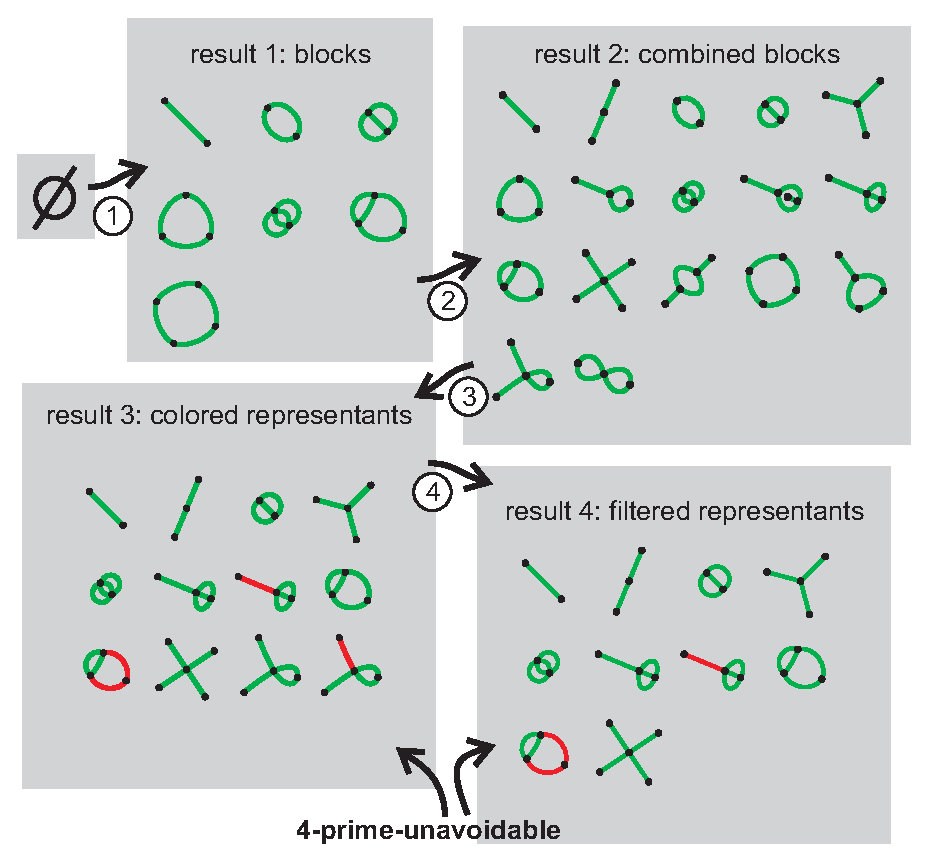
\includegraphics[width=12cm]{A.figs/unavoidablesetpipeline.eps}
   \end{center}
   \vspace{-0.7cm}
   \caption{Pipeline of the \kpu set generation for $k=4$}
   \label{fig:unavoidableSetPipeline}
\end{figure}

The \textsc{BlockGeneration} step has as input one positive integer $k$:
the maximum number of edges. Its output is all possible 2-connected
plane graphs with number of g-edges not exceeding $k$ plus the single-edge
plane graph. By convention we see all these plane graphs as
green-edged blinks. The blocks, besides the single-edged one, are
obtained from the plane graph with two parallel green edges shown on
Figure~\ref{fig:blockGeneration}A by applying inductively
and in all possible ways {\em vertex subdivisions} and
{\em face subdivisions}. An example of vertex subdivision may be seen on
Figure~\ref{fig:blockGeneration}B. Any two distinct angles on a
vertex are a base for this operation.  An example of face
subdivision may be seen on Figure~\ref{fig:blockGeneration}C.
Any two distinct angles on a face are a base for
this operation. For $k=4$, the number of resulting
blocks is 7 as it is shown on Figure~\ref{fig:unavoidableSetPipeline}.
The block term used here is also aligned to the fact that the
g-blinks induced from these resulting green-edged blinks do not
have breakpairs.
\begin{figure}[htp]
   \begin{center}
      \leavevmode
      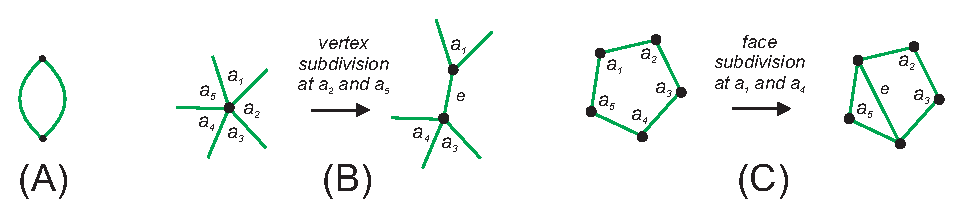
\includegraphics[width=12cm]{A.figs/blockgeneration.eps}
   \end{center}
   \vspace{-0.7cm}
   \caption{Block generation}
   \label{fig:blockGeneration}
\end{figure}

The \textsc{BlockCombination} step has as input $k$, the maximum number
of edges or g-edges, and the resulting blocks from the \textsc{BlockGeneration}
procedure. Here we see this input as green g-blinks and apply the
following algorithm. Let $B$ the set with these
input g-blinks or blocks. Make $A_1 = B$. For $i$ from 2 to $k$ make
$A_i$ the result of {\em combining} every g-blink at $A_{i-1}$ with each
g-blink in $B$. Combining a g-blink $G$ with $n_G$ g-zigzags to a
g-blink $G'$ with $n_{G'}$ g-zigzags results in $n_G \times n_{G'}$
g-blinks. This is the result of merging $G$ and $G'$ on
basepairs coming from all distinct combinations of g-zigzags. This
includes all possible spaces obtainable from merging $G$ and $G'$
as asserts Proposition~\ref{prop:sameZigzagsSameSpace}. The g-blinks
that overflows the maximum number of g-edges $k$ are discarded. For $k=4$,
the number of resulting combinations is 17 as it is shown on
Figure~\ref{fig:unavoidableSetPipeline}. Now we do an important
observation. Merging two g-blinks and then assigning a color to
each of its g-edges is the same as assigning the right colors in each
of the two g-blinks before merging and then merging them. This implies
that coloring the all-green g-blinks resulting from this step in all
possible ways really spans all possible spaces.

The \textsc{Coloring} step has as input the  all-green
g-blinks from the \textsc{BlockCombination} procedure.
The idea is to assign all possible g-edge color combination
to each of the given g-blinks. For each g-blink assigned
with a coloring some tests are made and this g-blink may
be discarded if it is asserted that, by doing this, we are
not losing a minimal g-blink to that same space (or its swapped
orientation version). Let $G$ be a g-blink already assigned
a coloring, these tests are the following:
\begin{enumerate}
\item If the number of red g-edges on $G$ is greater than the
number of green g-edges then it is discarded. This is
justified by the fact the red-green g-edges swapped version of $G$
will not be discarded by this rule (green g-edges is greater than
red g-edges) and it induces the same space as $G$ with orientation
changed.

\item If $G$ contains the structure shown
on the left side of Figure~\ref{fig:unecessaryGBlinkStructure}A it
is possible to apply a Reidemeister move of type II reducing by 2
the number of crossings and preserving the space. So $G$ is
unnecessary once its induced space was already considered by some
g-blink with fewer g-edges.

\begin{figure}[htp]
   \begin{center}
      \leavevmode
      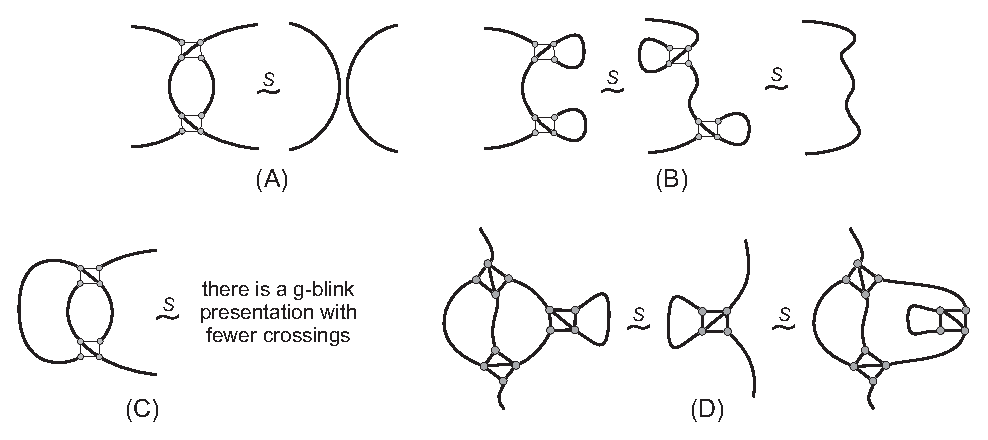
\includegraphics[width=12cm]{A.figs/unnecessarygblinkstructure.eps}
   \end{center}
   \vspace{-0.7cm}
   \caption{ Structures to identify g-blinks that may be discarded}
   \label{fig:unecessaryGBlinkStructure}
\end{figure}

\item If $G$ contains the structure shown
on the left side pattern or the middle pattern of
Figure~\ref{fig:unecessaryGBlinkStructure}B then it is unnecessary.
If it contains the left side pattern of
Figure~\ref{fig:unecessaryGBlinkStructure}B, by a ribbon move it is
converted to the pattern on the middle of
Figure~\ref{fig:unecessaryGBlinkStructure}B that may be converted by
Whitney Trick to the right pattern of
Figure~\ref{fig:unecessaryGBlinkStructure}B. All of them induce the
same space, and the right pattern has fewer crossings.

\item If $G$ contains the pattern on
Figure~\ref{fig:unecessaryGBlinkStructure}C then it has a {\em
circumcised component} and may be simplified by moves in the BFL
calculus to a g-blink with fewer crossings as it is explained on
pages 138--140 of \cite{KauffmanAndLins1994}. So, it may be discarded.

\item If $G$ contains the left or the right pattern on
Figure~\ref{fig:unecessaryGBlinkStructure}D then it may be simplified
by the move $K_4(1)$ of BFL calculus to the middle pattern with only
one crossing. So, it may be discarded.

\item If $G$ seen as a BFL contains more than one
component (more than one g-zigzag) and one of the components is completely
overcrossing the others or completely undercrossing the others than it may
be separated by Reidemeister moves and is not a minimal presentation.
\end{enumerate}
If g-blink $G$ passes all tests then one last transformation is done.
The g-blink included in the result set of this step is
actually $\min\{r(G), r(-G)\}$: the smallest g-blink
between the representative of $G$ or the representative of $-G$
\,\,(i.e. g-blink $G$ with all crossings changed (C) or, equivalently
all g-edge colors swapped). This resulting g-blink is asserted to
induce the same space as $G$ or its changed orientation version. Observe
that the g-blinks resulting from this step are all representatives.  For $k=4$,
the number of g-blinks resulting from this step is 12 (see
Figure~\ref{fig:unavoidableSetPipeline}).

The \textsc{Filtering} step has as input the representative
g-blinks resulting from the \textsc{Coloring} step. Let $B$ be this
input set and $R = \{\}$, initially empty, be the result set.
The filtering algorithm flows like this:


\begin{center}
 ALGORITMO
\end{center}

% {\setstretch{1.25}
% \begin{center}
% \hbox{
% \parbox{15cm}{
% \begin{small}
% \begin{algorithmic}[1]
%  \While{$B$ \, is not empty}
%     \State $G \leftarrow$ an element of $B$
%     \State $RM3 \leftarrow$ closure of $G$ by Reidemeiter III Move
%     \If{no element of $RM3$ may be discarded by rules 2 to 6 of the \textsc{Coloring} step}
%        \State $R \leftarrow R \cup \{G\}$
%     \EndIf
%     \State $B \leftarrow B \backslash RM3$
%  \EndWhile
% \end{algorithmic}
% \end{small}}}\end{center}
% }
The idea of this step is to use the Reidemeister III move, that preserves
the number of crossings and the space, to find some blink version of the
space that may be simplified by the rules 2 to 6 explained on the
\textsc{Coloring} step. If there exists such a version then that
g-blink and the whole closure of g-blinks obtained from it by
Reidemeister III may be discarded. Otherwise only the given
g-blink on its Reidemeister III closure may be preserved (that
is why we remove all RM3 set on line 7 of the above algorithm).
The result of this step for $k = 4$ is a set with 10 g-blinks
(see Figure~\ref{fig:unavoidableSetPipeline}).

We name $U$ the set resulting from this pipeline for $k=9$. This set
is, as we saw in its construction, a \hbox{\npu{9}} set and has 3437 g-blinks
divided in 1 g-blink with 1 g-edge, 1 g-blink with 2 g-edges, 2 g-blinks
with 3 g-edges, 6 g-blink with 4 g-edges, 12 g-blinks with 5 g-edges, 43
g-blinks with 6 g-edges, 133 g-blinks with 7 g-edges, 585 g-blinks with
8 g-edges and 2654 g-blinks with 9 g-edges. We denote by $U[1]$ the
smallest g-blink in $U$, $U[2]$ the second smallest g-blink in $U$,
up to $U[3437]$ the greatest g-blink in $U$. The time elapsed to
generate the set $U$ was less than twelve hours. At this point we have
the first two ingredients to a census of prime spaces up to 9 g-edges:
$(9, U, ?)$. The only missing part is the third ingredient of a census:
the partition function. This is the subject of next section.

\subsection{Topological classification of g-blinks in $U$}
\label{sec:topologicalClassificationOfU}

The set $U$ is a \npu{9} set of g-blinks. The next step to define
a census of prime spaces with a g-blink (or blinks) presentation
with up to 9 g-edges (edges) is to identify what g-blinks induce
different spaces and what g-blinks induce the same space
(modulo the orientation). To reach
this goal the first thing we did was to
calculate, for each g-blink in $U$, the homology group and the
Witten-Reshetikhin-Turaev quantum invariant (for
$r \in \{3,4,5,6,7,8\}$) of its induced space. In
Sections~\ref{sec:homologyGroup}~and~\ref{sec:quantumInvariant}
we show how to do this calculation from a g-blink
presentation of a space. To help on this exposition
we will use HG, QI and HGQI when we want to refer
to the homology group, quantum invariant, respectively.
The time elapsed to calculate the HG and QI of all
g-blinks in $U$ was less than half an hour.

The effect on the quantum invariant of changing the
orientation of a space is that each complex number in
its sequence becomes its conjugate (remember that the
quantum invariant is a sequence of complex numbers). So
when two g-blinks have their QIs differing by, for each
$r$, one being the conjugate of the other, then these
g-blinks may induce the same space in different
orientations. As it was defined for a census, g-blinks
that induce distinct orientations of the same space are
mapped, by the partition function, to the same value. We
are interested in spaces modulo orientations. For this
reason, we mounted from the HG and QI data of each
g-blink in $U$ the information named HGnQI (HG and
normalized QI). It is just the pair HG and nQI where
nQI is the normalized version of QI: if the first complex
entry with imaginary part in QI is negative then nQI
entries are the conjugate of QI entries, otherwise nQI
is equal to QI.

Using the HGnQI information of each g-blink we partitioned the
set $U$ into 501 classes. The 3437 g-blinks of $U$ induced 501
distinct HGnQIs. One consequence of this fact is that $U$ induces, at
least, 501 different (modulo orientation) spaces. This HGnQI partition
of the set $U$ is a first candidate for the partition function
to the census we want. If the homology group together with
the quantum invariant is a strong enough invariant of space,
then we already have the exact partition function we want. To
prove this, it remains to show that all entries in the
same HGnQI class indeed induce the same space. To do
this, we need another tool. Before entering into this topic,
we want to make some comments about the HGnQI partition of $U$.

After partitioning the set $U$ in HGnQI classes, a very apparent
fact was that the quantum invariant was almost perfect in
identifying the 501 classes. It, alone, separated $U$ into 498
classes. In only 3 cases the homology group was important to
distinguish spaces that the quantum invariant did not. In
Figure~\ref{fig:qiFailure} we show a blink presentation for
these 3 cases.
\begin{figure}[htp]
   \begin{center}
      \leavevmode
      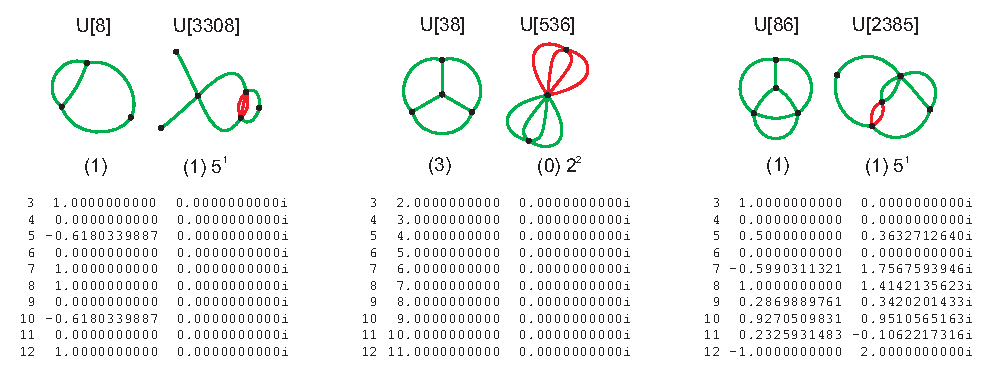
\includegraphics[width=15cm]{A.figs/qifailure.eps}
   \end{center}
   \vspace{-0.7cm}
   \caption{ The 3 cases in $U$ where HG helped QI to distinguish spaces}
   \label{fig:qiFailure}
\end{figure}
In the first case, $U[8]$ has HG $(1)$
while $U[3308]$ has HG $(1) 5^1$ and the 12 first
entries of the quantum invariants, as is shown,
are all real numbers. Indeed, all entries in the QI of $U[8]$
sequence are real once it has only one orientation.
For a proof of this fact note that
$\textsc{Dual}(U[8])$ is $U[8]$ with
all edges being red which is also $U[8]$ after applying (C)
(change crossings). As these two g-blinks are the same
g-blink and they are the two possible orientations
for the space, we can conclude that this space has only
one orientation. In the second case, $U[38]$ has HG $(3)$
while $U[536]$ has HG $(0) 2^2$ and the 12 first
entries of the quantum invariants, as is shown,
are all integer numbers. In the third case, $U[86]$ has HG $(1)$
while $U[2385]$ has HG $(1) 5^1$ and the 12 first
entries of the quantum invariants, as is shown,
are all complex numbers. It might be the case that
the quantum invariant in some point distinguishes these
spaces as the homology group did. We did not check this.

Now let's return to our open problem. Are the 501 HGnQI
classes really inducing the same space or some of them
induce more than one space? To answer this question we
used 3-gem theory. We saw in Section~\ref{sec:fromGBlinkTo3Gem}
that from a g-blink we can obtain a 3-gem inducing the
same space as it does. This fact enables us to change
our question in g-blink language into a question in 3-gem language. The
idea is to take, for each of the 501 HGnQI classes, all g-blinks
in the same HGnQI class, calculate a 3-gem version for it
and then try to find a proof that they are the same space, i.e.
a path of ``moves'' in 3-gems that preserve the induced space
connecting all these 3-gems.

% \newcommand{\GemOfGBlink}{
% \parbox{7.5cm}{
% \begin{footnotesize}
% \setstretch{1.25}
% \begin{algorithmic}[1]
%    \Function{GemOfGBlink}{$G$}
%    \State $J \leftarrow \textsc{GBlink2Gem}(G)$
%    \While{true}
%       \State $\textsc{SimplifyGem}(J)$
%       \State $\textsc{SearchInTSClass}(J,12\, {\rm seconds})$
%       \If{$J$ has no dipole, no $\rho_2$-pair and no $\rho_3$-pair}
%          \State break
%       \EndIf
%    \EndWhile
%    \State {\bf return} \,\, $J$
%    \EndFunction
% \end{algorithmic}
% \end{footnotesize}
% }}
% 
% \newcommand{\SearchInTSClass}{
% \parbox{7.5cm}{
% \begin{footnotesize}
% \setstretch{1.25}
% \begin{algorithmic}[1]
%    \Procedure{SearchInTSClass}{$J, maxtime$}
%       \State $C \gets \{ J \}$ \,\, $U \gets \{ J \}$ \Comment{$C$ is the current TS-class of $J$ and $U$ are the unprocessed gems}
%       \While{$U$ is not empty and elapsed time < $maxtime$}
%          \State $J' \leftarrow$ a gem in $U$
%          \State $U \leftarrow U \backslash \{J'\}$
%          \For{all possible TS-moves $m$ in $J'$ }
%             \State $J'' \leftarrow J'$ with TS-move $m$ applied
%             \If{$J'' \notin C$}
%                 \If{there is a dipole or $\rho_2$-move or $\rho_3$-move in $J''$}
%                     \State $J \gets J''$ and exit
%                 \Else
%                     \State $U \leftarrow U \cup \{J''\}$
%                     \State $C \leftarrow C \cup \{J''\}$
%                 \EndIf
%             \EndIf
%          \EndFor
%       \EndWhile
%       \State $J \gets \min\{J'\in C\}$
%    \EndProcedure
% \end{algorithmic}
% \end{footnotesize}
% }}
% 
% \newcommand{\SimplifyGem}{
% \parbox{7.5cm}{
% \begin{footnotesize}
% \setstretch{1.25}
% \begin{algorithmic}[1]
%    \Procedure{SimplifyGem}{$J$} \Comment{$J$ becomes its simplified version}
%    \While{true}
%       \If{there is a dipole in $J$}
%          \State apply dipole cancelation in $J$
%       \ElsIf{there is a $\rho_3$-pair or $\rho_2$-pair in $J$}
%          \State apply $\rho_3$-pair or apply $\rho_2$-pair in $J$
%       \Else  \State break
%       \EndIf
%    \EndWhile
%    \EndProcedure
% \end{algorithmic}
% \end{footnotesize}
% }}

The 3-gem that we associated to each g-blink in $U$ was given by
the function \textsc{GemOfGBlink} shown in Algorithm \ref{alg:algorithmFor3Gems}.
The idea of this function is to simplify the initial 3-gem of
the g-blink given by the \textsc{GBlink2Gem} procedure explained in
Section~\ref{sec:fromGBlinkTo3Gem} using dipole cancelations,
$\rho_2$-moves, $\rho_3$-moves and TS-moves until it cannot be simplified
anymore or until a certain timeout occurs. This step resulted in 999
distinct gems for the 3437 g-blinks of $U$. We used a timeout of 12 seconds.
From these 999 3-gems, 657 (or 65\%) gems were proven to be
TS-class representatives (minimum 3-gem in the class) such that the entire class
had no simplifications of the types: dipole cancelation, $\rho_2$-move and $\rho_3$-move.
The remaining 342 3-gems were the minimum 3-gem obtained before the timeout
occurred. The 3-gem also encodes the orientation of the space, but, in
this case we used 3-gems modulo orientation. In other words, the 3-gem we
associated to each g-blink could be exactly the same space, or the same
space with orientation changed. As it might be clear now, this is enough
here: spaces modulo orientation.
% \begin{algorithm}
% \caption{Algorithms for 3-Gems}
% \label{alg:algorithmFor3Gems}
% \smallskip
% \begin{tabular}{c|c}
% \begin{tabular}{c}
% \GemOfGBlink\\[2.9cm] \hline
% \\[-0.05cm]
% \SimplifyGem
% \end{tabular} &
% \SearchInTSClass
% \end{tabular}
% \end{algorithm}

\center{ACIMA TEM UM ALGORITMO}\\

The remaining challenge at this point was to find whether these 999
3-gems, seen as nodes of a graph, could be connected in 501
connected components, where a connected component means that all
gems in the same component induce the same space (modulo
orientation). So, we started to insert edges in this graph of 999
nodes and initially no edge. This was done by ``perturbing'' the
gems on the nodes by using U-moves and then applying the same
simplification procedure used in the function \textsc{GemOfGBlink}
until a gem with no simplification or a timeout occurred. This final
gem, if not yet in our graph, was added as a new node. An edge, if
not existent, from the perturbed 3-gem node to this new, or already
existent, node, was also added to the graph. This procedure was
oriented by the HGnQI classes, so if a HGnQI class was already a
single connected component then nothing more was needed to be done
there: the HGnQI class was proved to be a single space (modulo
orientation). This procedure of connecting the gems of a HGnQI class
on this graph took about 3 days with manual interference being
important: by looking at the graph we perturbed the most promising
nodes. The final result was: 499 of the 501 HGnQI classes were
proven to induce a single space (modulo orientation). In only two
HGnQI classes we could not find a single connected component.

\begin{figure}[htp]
   \begin{center}
      \leavevmode
      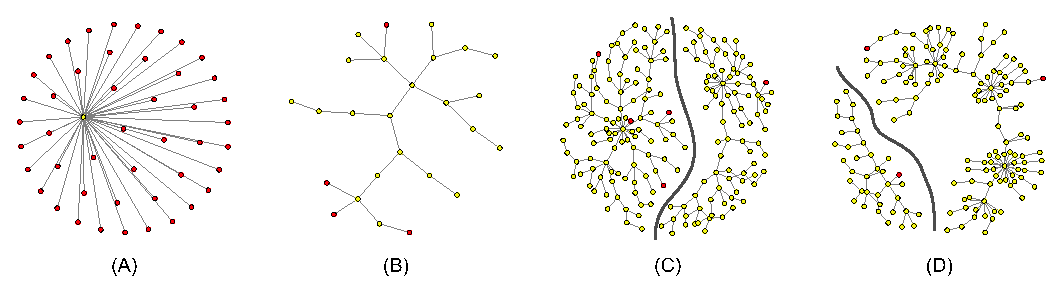
\includegraphics[width=15cm]{A.figs/subgraphs.eps}
   \end{center}
   \vspace{-0.7cm}
   \caption{Graphs of g-blinks (red nodes) and gems (yellow nodes). The first two are trees
   and the last two are forests with two components (the two uncertainties)}
   \label{fig:subgraphs}
\end{figure}

Figure~\ref{fig:subgraphs} shows subgraphs (trees) for 4 HGnQI
classes on the final graph. The red nodes are g-blinks from $U$. The
yellow nodes are the 3-gems. Note that every red node is connected
to a single yellow node: this yellow node is the result of the
\textsc{GemOfGBlink} applied to this g-blink.
Figure~\ref{fig:subgraphs}A was an easy case where all g-blinks
of the same HGnQI class were pointing right to the same 3-gem.
Nothing was needed to do in this case. Figure~\ref{fig:subgraphs}B
was one of the difficult cases: many redundant edges (not shown) and
different 3-gems were generated before all g-blinks were connected.
\begin{figure}[htp]
   \begin{center}
      \leavevmode
      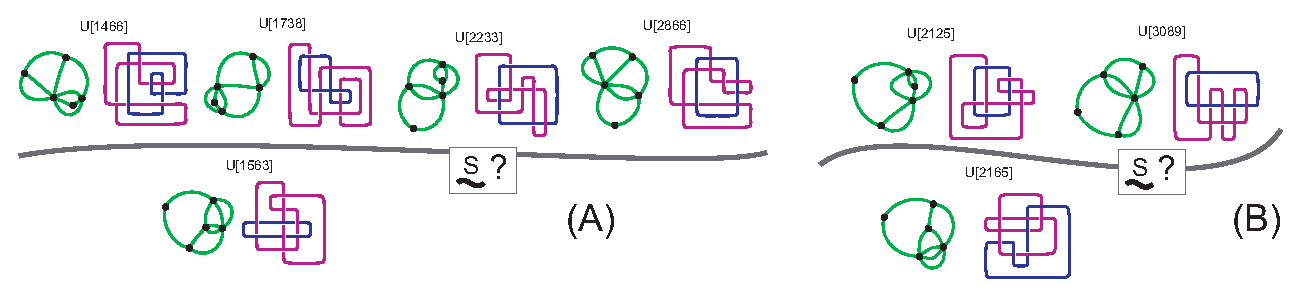
\includegraphics[width=16cm]{A.figs/doubts.eps}
   \end{center}
   \vspace{-0.7cm}
   \caption{ The only 2 classes with same HGnQI where a proof of the homeomorphism was not found}
   \label{fig:doubts}
\end{figure}

Figures~\ref{fig:subgraphs}C~and~\ref{fig:subgraphs}D presents the
two cases where one doubt was left. In each of these cases, two
connected components remained: they are shown with the dark line
separating them. In the first case, Figure~\ref{fig:subgraphs}C, the
HGnQI class had 5 g-blinks where 4 of them were proven to be the
same space. In the second case, the HGnQI class had 3 g-blinks where
2 of them were proven to induce the same space. A blink and BFL
presentation for the g-blinks involved in these doubts are shown in
Figure~\ref{fig:doubts}. In the first doubt, the g-blinks involved
are $U[1466]$, $U[1563]$, $U[1738]$, $U[2233]$, $U[2866]$ and
$U[1563]$ is the only g-blink we did not find a proof as being the
same space (modulo orientation) of the others. In the second doubt,
the g-blinks involved are $U[2125]$, $U[2165]$, $U[3089]$ and
 $U[2165]$ is the only g-blink we did not find a proof as
being the same space of the others. Is there a proof for these
two cases and we just could not find them or are these the only
weak points of the HGnQI invariant on the set $U$? We leave
this question open and register it as the following conjectures.

\begin{conjecture} \label{conj:conjecture1}
The spaces induced by all 5 blinks or BFLs on Figure~\ref{fig:doubts}A
are the same.
\end{conjecture}

\begin{conjecture} \label{conj:conjecture2}
The spaces induced by all 3 blinks or BFLs on Figure~\ref{fig:doubts}B
are the same.
\end{conjecture}

The only reason we conjecture these stems from the fact that
HGnQI have not failed in all other 499 cases. But,
the fact that we had no success, after various days of
computational effort trying to prove these conjectures
using the simplification combinatorial dynamics of 3-gems,
suggests the contrary: these conjectures are false.
Figures~\ref{fig:subgraphs}C~and~\ref{fig:subgraphs}D show the
two trees that could not be connected for
each case after all the computational effort.

All data involved in all the experiments we explained here are in a computer program named
\textsc{Blink}. So a proof that all HGnQI classes indeed induce the same space,
except for the two cases explained, can be exhibited by this program.

\enlargethispage{0.5cm}
In the 3-gem presentation it is sometimes possible to identify that
its induced space is composite. For example the space induced by g-blink $U[31]$
is also induced by a 3-gem ($r_4^{18}$ in the 3-gems catalogue of \cite{Lins1995}) that
contains a {\em disconnecting quartet}, i.e. four edges with distinct colors
that disconnected the 3-gem. The existence of this structure in a 3-gem
or the existence of handles, i.e. connected sums with $\mathbb{S}^2 \times \mathbb{S}^1$,
is a proof that the induced space is composite. In the 501 HGnQI classes, using
this kind of 3-gem information, we could prove that 14 of them were composite. The
rules that we used in the construction of $U$ were not able to identify that
some g-blinks induced composite spaces, but, anyway, that was not the goal there. The
goal there was to create a small set of g-blinks that did not lose a minimal
presentation by g-blink of a prime space. This is the important property of $U$:
all prime spaces have a minimal g-blink presentation in $U$. Using this information
of the 14 composite classes, we named each of the 501 HGnQI classes like this:
the 487 classes that were not proven composite gained names 1.1, 2.1, 3.1  $\ldots$  3.2,
4.1 $\ldots$ 4.5, 5.1 $\ldots$ 5.6, 6.1 $\ldots$ 6.19, 7.1 $\ldots$ 7.38, 8.1 $\ldots$ 8.119
and 9.1 $\ldots$ 9.296; the 14 classes that were proven composite gained names 6.1c \ldots 6.3c,
8.1c \ldots 8.5c and 9.1c $\ldots$ 9.6c. The number before the point stands for
the number of g-edges of the minimal g-blink in $U$ found for that space.
Let $U[n.i]$ denote the smallest g-blink (i.e. smallest code) in class $n.i$, i.e.
$U[n.i] = \min\{G \in n.i\}$. For instance $U[5.1]$ is $U[11]$ and $U[6.1{\rm c}]$ is $U[31]$.
The number after the point stands for the following: $n.1$ is the class
where g-blink $U[n.1]$ has $n$ g-edges and is the smallest g-blink among all
classes $U[n.j]$, for any $j$ that defines a valid class name; $n.2$ is the class
where g-blink $U[n.2]$ has $n$ g-edges and is the second smallest g-blink among all
classes $U[n.j]$, for any $j$ that defines a valid class name; and so on. The two
classes that we do not know whether they induce a single space or two spaces are 9.126
(Figure~\ref{fig:doubts}A) and 9.199 (Figure~\ref{fig:doubts}B).

\begin{figure}[h!tp]
   \begin{center}
      \leavevmode
      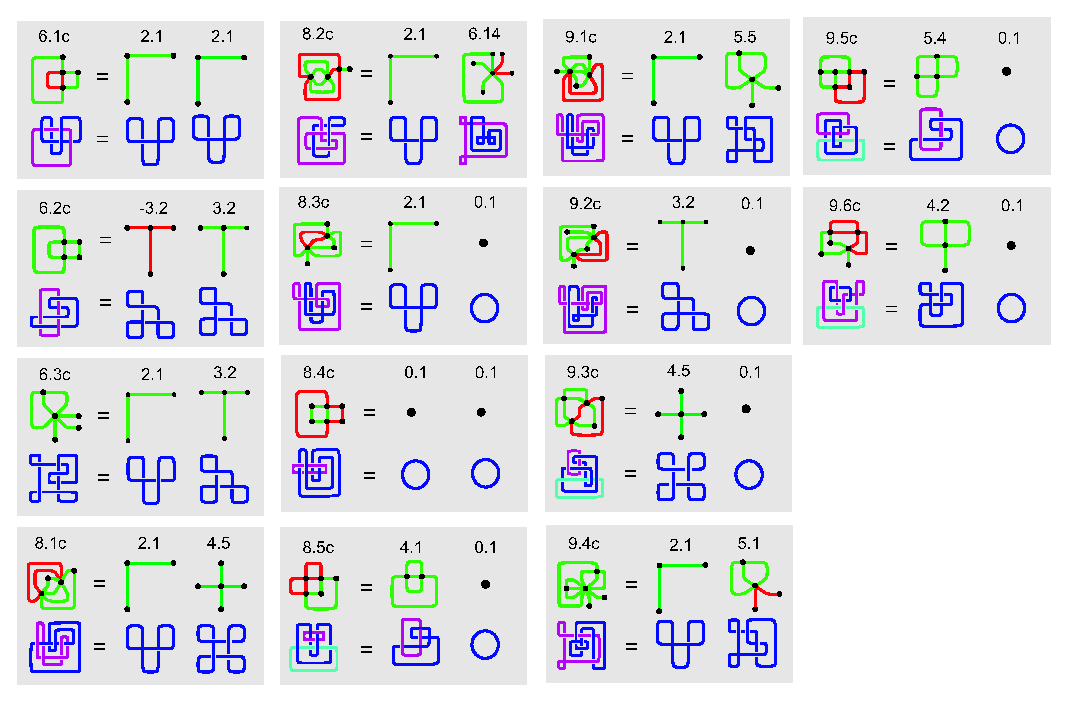
\includegraphics[width=16cm]{A.figs/compositespaces.eps}
   \end{center}
   \vspace{-0.7cm}
   \caption{ The 14 composite spaces in $U$}
   \label{fig:compositeSpaces}
\end{figure}

The 14 composite spaces in $U$ are in Appendix~\ref{chap:compositeCatalogue}.
The quantum invariant at level $r$ of the connected sum of spaces $A_1 \ldots A_n$ is the product
of their quantum invariants at the same level divided by the $r$-th quantum invariant of $\mathbb{S}^3$ to
the power $n-1$. Using this we could align the orientations of the prime spaces that
produced these composite spaces. Figure~\ref{fig:compositeSpaces} shows explicitly these
14 spaces as a prime space composition with the correct orientation.

The space $\mathbb{S}^2 \times \mathbb{S}^1$ has a blink presentation that is just a vertex
and no edges, i.e. a BFL that has no crossings and is just a closed loop. This
space is a special one as it is the only prime space that has a blink presentation
without edges. By the rules we used on the construction of set $U$ this space
needed not to appear once: (1) we did not include blinks without edges and
(2) only one minimal presentation of a space was asserted to appear. This
space should be included artificially after. In spite of that, $\mathbb{S}^2 \times \mathbb{S}^1$
appeared as class 6.5. Figure~\ref{fig:gblinksForS1xS2inU} shows a blink
and a BFL for the 36 g-blinks in class 6.5. In a strict sense, this class
could be named 0.1 and spaces 6.6 to 6.19 would be decreased by one to 6.5
to 6.18, but we do not do this.

\begin{figure}[h!tp]
   \begin{center}
      \leavevmode
      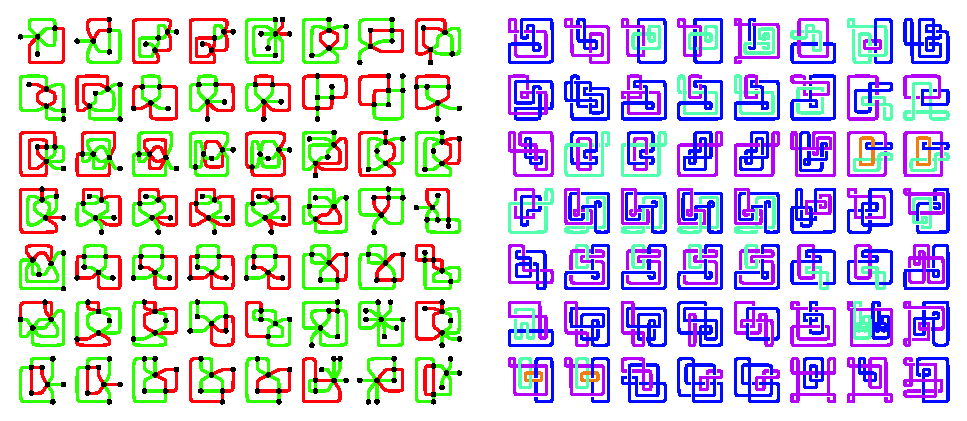
\includegraphics[width=14cm]{A.figs/gblinksfors1xs2inu.eps}
   \end{center}
   \vspace{-0.7cm}
   \caption{ Blink and BFL presentations for g-blinks in 6.5: space $\mathbb{S}^2 \times \mathbb{S}^1$}
   \label{fig:gblinksForS1xS2inU}
\end{figure}


\begin{theorem}
\label{theo:primeSpacesUpTo9Edges}
Any prime space that has a blink presentation with $\leq$ 9 edges induces the
same space (modulo orientation) as one and only one of the 487 blinks in
Figure~\ref{fig:primeSpace487Representatives} or the 487 BFLs in
Figure~\ref{fig:primeSpace487RepresentativeLinks} or the 487 spaces shown
in Appendix~\ref{chap:primeCatalogue}.
\end{theorem}

\enlargethispage{2cm}

\begin{proof}
The construction of set $U$ asserts that it contains at least one minimal
g-blink for each prime space except for space $\mathbb{S}^2 \times \mathbb{S}^1$,
which is a special case where its minimal blink presentation
has no edges: only a single vertex. In spite of that $\mathbb{S}^2 \times \mathbb{S}^1$
appears in $U$ as class 6.5 so any prime space is included. The proof
that there are only 487 (with 2 doubts) is in the program \textsc{Blink}.
\end{proof}

A closed compact oriented 3-manifold is {\em $n$-small} if it is induced by a blink with
at most $n$ edges.

\newpage

\begin{figure}[h!tp]
   \begin{center}
      \leavevmode
      %\includegraphics[width=14.5cm]{A.figs/primeSpace487Representants.eps}
      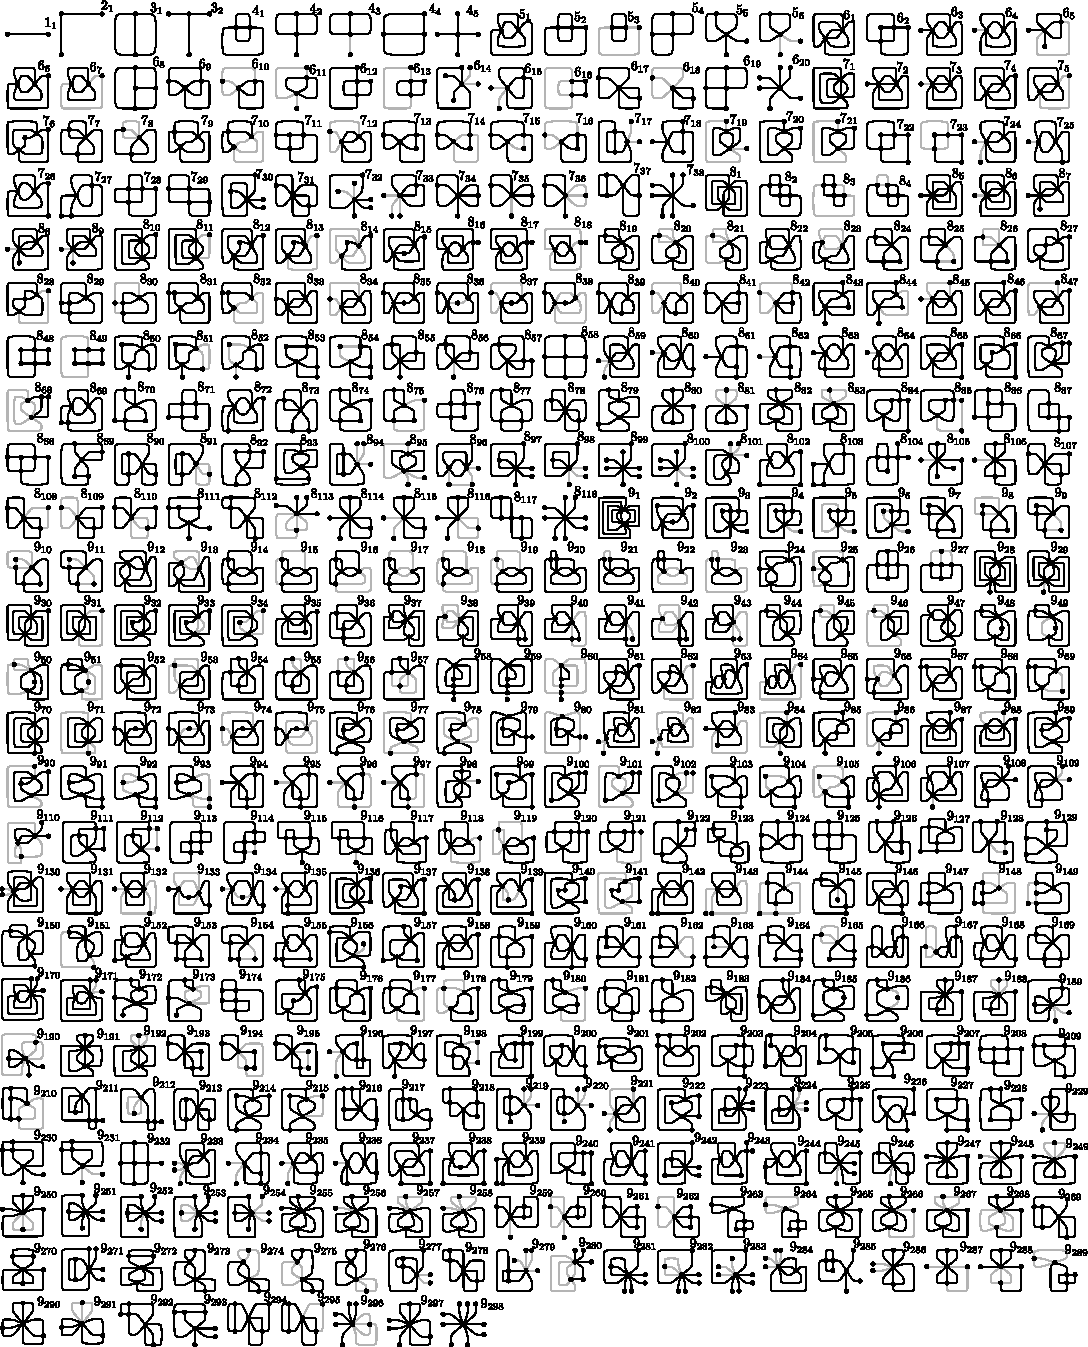
\includegraphics[height=22.5cm]{E.figsbw2/primespace487representants_bw.pdf}
   \end{center}
   \vspace{-0.7cm}
   \caption{A complete topological census of 9-small closed oriented 3-manifolds}
   \label{fig:primeSpace487Representatives}
\end{figure}

\newpage

\begin{figure}[h!tp]
   \begin{center}
      \leavevmode
      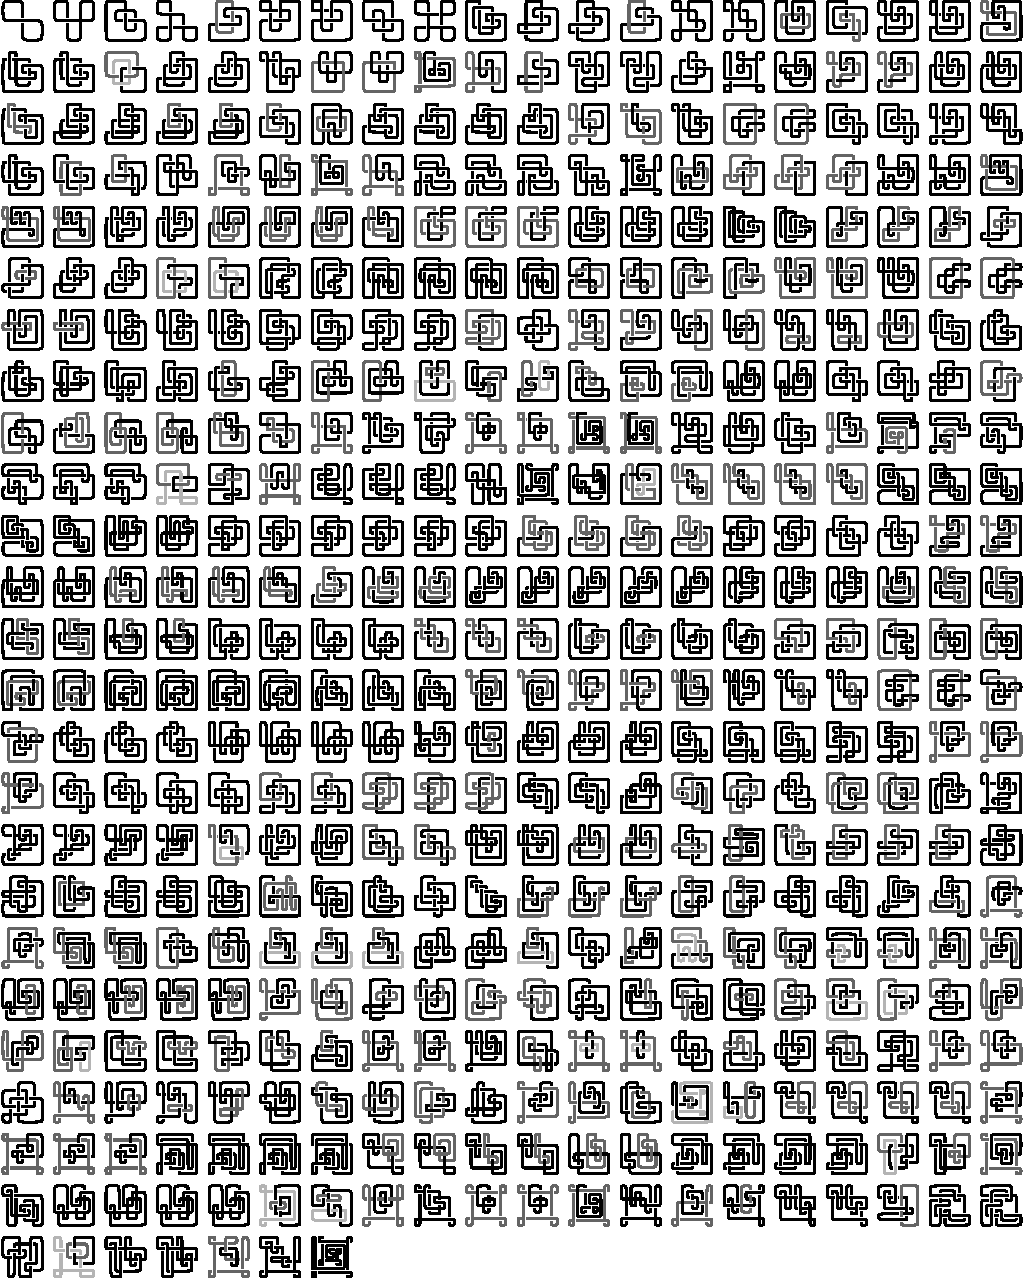
\includegraphics[height=22.0cm]{E.figsbw2/primespace487representantlinks_bw.pdf}
   \end{center}
   \vspace{-0.7cm}
   \caption{Corresponding links for the topological census of 9-small 3-manifolds}
   \label{fig:primeSpace487RepresentativeLinks}
\end{figure}

\newpage

\subsection{Spaces induced by simple 3-connected monochromatic blinks}

Blinks bring to the stage a very interesting connection: spaces and
plane graphs. Can concepts of graph theory when interpreted in space
language bring light to some unknown aspect of spaces? Some new
invariant for spaces?

With this spirit, what can we say about the space of a blink that is
$k$-connected? In Chapter~\ref{chap:blinks} we saw that the blocks
(2-connected pieces) of a blink may be recombined in different
ways leading to the same space. What are these blocks?
In this crude form, this concept of block or more general
$k$-connected blink does not mean something useful in
the language of spaces because of the following
observation: using the $B_2$ move of blink calculus
(i.e. $RM_2$ in BFL calculus) explained
on Section~\ref{sec:blinkCalculus} one
may obtain blinks with higher connectivity inducing
the same space. But this comes
at a price, these equivalent versions with higher
connectivity contains local simplifications (moves
that reduce the number of edges) that leads back to
the first blink we started. A family of blinks
that do not contain these local simplifications are the
monochromatic blinks. Note that all simplification moves
on the blink calculus shown in Section~\ref{sec:blinkCalculus}
are, except for $B_4(1)$, from pieces with two colors. When
talking about blocks or higher connected monochromatic
blinks there is no local simplification at all.
So, the connectivity issue on monochromatic blinks
might mean something on spaces.

\begin{figure}[htp]
   \begin{center}
      \leavevmode
      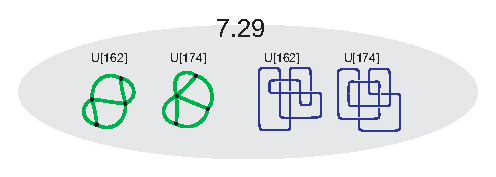
\includegraphics{A.figs/nontrivialgreenblocks.eps}
   \end{center}
   \vspace{-0.7cm}
   \caption{ Non-trivial pair of green blocks (2-connected blinks) inducing the same space}
   \label{fig:nonTrivialGreenBlocks}
\end{figure}

Let $B$ be a green (all edges green) blink, $B'$ be a green blink
whose map (plane graph) is the dual map of $B$, $B''$ be $B$
reflected on the plane and $B'''$ be $B'$ reflected on the plane.
As we saw in Chapter~\ref{chap:blinks} all these blinks induce the
same space modulo orientation. Let's denote as {\em trivial}
a pair of blinks $A$ and $B$ if they induce the same space modulo
orientation and $A \in \{B,B',B'',B'''\}$. A pair of blinks inducing
the same space modulo orientation that is not trivial is called
{\em non-trivial}. Are all pair of green blocks (2-connected blinks)
that induce the same space modulo orientation trivial?
No. Space $7.29$ in Appendix~\ref{chap:primeCatalogue}
has a counterexample. Figure~\ref{fig:nonTrivialGreenBlocks} shows
a pair of non-trivial green 2-connected blinks in space 7.29 that induces
the same space. By the fact that they  all induce the same space, there must exist
paths connecting these blinks (or BFLs) using the moves
on the blink calculus (or BFL
calculus). Can you find such a path? We found the path via gem theory.

What about simple 3-connected monochromatic blinks?  Are there
non-trivial pairs of simple 3-connected monochromatic blinks?
To answer this question we generated a set named $T$ with all simple
3-connected green blinks up to 16 edges\footnote{To generate the simple
3-connected maps we started from the wheel maps (maps that are a polygons
with its vertices connected to a central vertex) and then, inductively, we
subdivided the faces and vertices in all possible ways preserving the
3-connectivity property.}
and calculated their HGnQI invariants (QI up to level 8).
The result was interesting. There are
708 simple 3-connected monochromatic g-blinks and they are divided in 381
classes HGnQI. These classes were named: $6.1$t, $8.1$t, $9.1$t,
10.1t$\ldots$ 10.2t, 11.1t $\ldots$ 11.2t, 12.1t $\ldots$ 12.9t,
13.1t $\ldots$ 13.11t, 14.1t $\ldots$ 14.36t, 15.1t $\ldots$ 15.76t
and 16.1t $\ldots$ 16.242t. This name convention is analogous to
the convention of the HGnQI classes in $U$ except for the
letter ``t'' at the end. These classes are presented with details in
Appendix~\ref{chap:catalolgue3con}. In these 381 classes there are
only 11 classes with exactly one non-trivial pair candidate. They
are shown in Figure~\ref{fig:doubts3ConnectedIsolated}.

\enlargethispage{2cm}

\begin{figure}[htp]
   \begin{center}
      \leavevmode
      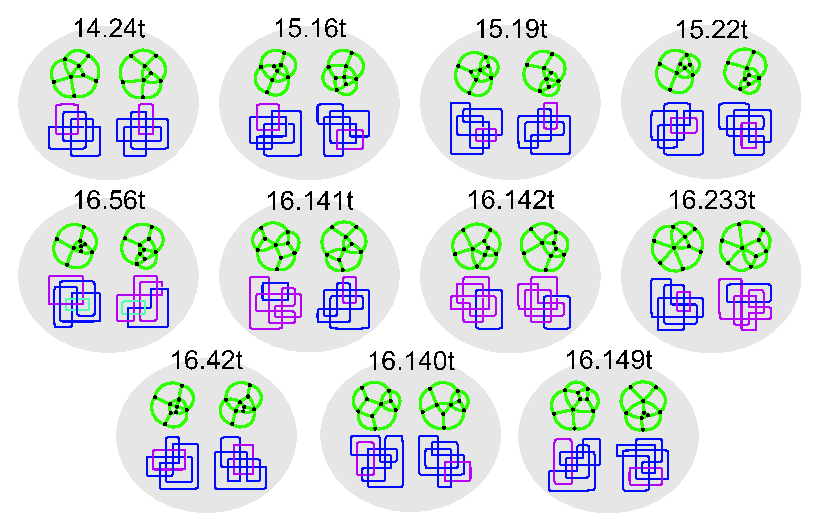
\includegraphics{A.figs/doubts3connectedisolated.eps}
   \end{center}
   \vspace{-0.7cm}
   \caption{ Doubts on simple 3-connected all green blinks}
   \label{fig:doubts3ConnectedIsolated}
\end{figure}

Is any of these a non-trivial pair or all of them induce different spaces
modulo orientation that the HGnQI could not capture? We leave this question
open.
